\chapter{Chaos analysis of the electronic Burridge-Knopoff model}\label{chap: chaos analysis}


\section{Chaos analysis of two coupled blocks}\label{sec: 2 blocks chaos}

Relying on the tools that have been introduced in Chapter~\ref{chap: chaos},
it is possible to analyze the chaotic behavior of a system starting from a time series.
Considering the electronic implementation of the Burridge-Knopoff model that has been discussed
in Chapter~\ref{chap: electronic analog of bk}, we can thus analyze the double block behavior
of the circuit (see Section~\ref{sec: double block characterization}).

The time series $y_n$ was chosen to be the signal $W_1$ (see Fig.~\ref{fig: circuit diagram}),
which was sampled for 10 s with a sampling time of 0.1 ms, resulting in $10^5$ points in the sequence.
The driving voltage $V_d$ was set to 0.05 V, since the chaotic behavior seems present only for
$V_d \lesssim 0.11$ V (see Fig.~\ref{fig: bifurcation}). The results of the application of the
``chasing chaos'' method described in Section~\ref{sec: method for chaos} are shown in Fig.~\ref{fig:2 blocks chaos}.

\begin{figure}[h!]
    \centering
    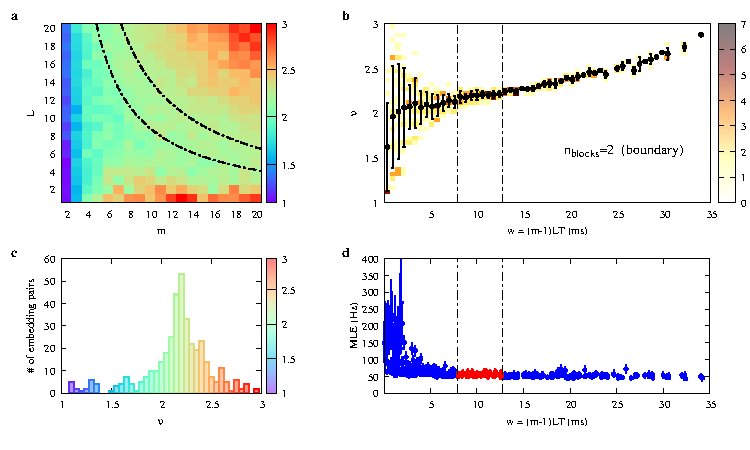
\includegraphics[width=\linewidth]{../blocks/2_blocks/1e5_points/plots/chaos.pdf}
    \caption{``Chasing chaos'' analysis of the experimental $W_1$ time series
    obtained by setting $V_d=0.05$ V with 2 coupled blocks.
    The number of elements in the sequence is $10^5$.
    (a) Map of estimated correlation dimension $\nu$ vs.\ embedding pair $(m, L)$.
    The black, dash-dotted hyperbolae bound the region of uniform $\nu$ corresponding to the interval of the
    embedding window $w$ highlighted in (b) and (d).
    (b) Sample joint distribution of $(w,\nu)$ for the $\nu$-map in (a).
    Black dots and the related errobars correspond to the expected value and the related uncertainty of $\nu$
    for each given value (bin) of $w$. A uniformity region, highlighted by the dash-dotted vertical lines,
    is identified. (c) Histogram of the estimated $\nu$. (d) Distribution of MLE as a function of $w$. Each point and the related
    uncertainty corresponds to the value assessed on an embedding pair by using the divergence rate method.
    A cluster of points, marked in red, can be identified in the uniformity region of (b), also highlighted here.
    }\label{fig:2 blocks chaos}
\end{figure}

In Fig.~\ref{fig:2 blocks chaos}a the heatmap of the correlation dimension $\nu$ in the embedding
lattice is shown. The two hyperbolae bound the uniformity region, which was chosen by searching for
a plateau in the joint distribution in Fig.~\ref{fig:2 blocks chaos}b.
Carrying out a weighted average of the correlation dimension estimates in the uniformity region yields
$\nu=2.20\pm0.02$, which complies with the peak of the histogram in Fig.~\ref{fig:2 blocks chaos}c,
which is $2.20\pm0.05$.

The estimates of the maximum Lyapunov exponent as a function of the embedding window are shown in
Fig.~\ref{fig:2 blocks chaos}d. Carrying out another weighted average of the MLE in the uniformity region
yields $\text{MLE}=(54\pm1)$ Hz. Since the uniformity region is easy to be identified, it is reasonabl
to conclude that this system is chaotic.
Nonetheless, the estimates of $\nu$ and MLE are assumed to be valid.

This chaos analysis was carried out also on a breadboard implementation of the circuit~\cite{ref:electronic_analog}.
A uniformity region was identified and the correlation dimension was found to be
$\nu=1.971\pm0.007$. Regarding the MLE, a cluster of values at about 45 Hz occurred, which complied
with the numerical value $\text{MLE}=(46\pm5)$ Hz, which was found integrating the differential
equations of the system (Eq.~\ref{eq: 2 block motion electronic}) and applying the so-called
standard method~\cite{benettin1980lyapunov1,benettin1980lyapunov2}.

Both the estimates for the correlation dimension and the maximum Lyapunov exponent are larger
in the integrated board case with respect to the breaboard case.
A possible explanation for this is the higher presence of noise in the integrated board;
as was discussed in Section~\ref{subsec: testing the procedure}, the correlation dimension evaluation
increases with noise.

Nevertheless, the chaotic dynamics is observed in both implementations. The calculations of $\nu$ and
MLE strongly depend on many factors, such as the embedding lattice, the sampling time, or the
arbitrariness on the choice of the uniformity region.
Thus, the results on the two implementations are assumed to be in compliance with each other.


\section{Chaos analysis of three coupled blocks}\label{sec: 3 blocks chaos}




